%%%%%%%%%%%%%%%%%%%%%%%%%%%%%%%%%%%%%%%%%%%%%%%%%%%%%%%%%%%%%%%%%%%%
%% I, the copyright holder of this work, release this work into the
%% public domain. This applies worldwide. In some countries this may
%% not be legally possible; if so: I grant anyone the right to use
%% this work for any purpose, without any conditions, unless such
%% conditions are required by law.
%%%%%%%%%%%%%%%%%%%%%%%%%%%%%%%%%%%%%%%%%%%%%%%%%%%%%%%%%%%%%%%%%%%%

\documentclass[
  digital, %% The `digital` option enables the default options for the
           %% digital version of a document. Replace with `printed`
           %% to enable the default options for the printed version
           %% of a document.
%%  color,   %% Uncomment these lines (by removing the %% at the
%%           %% beginning) to use color in the digital version of your
%%           %% document
  table,   %% The `table` option causes the coloring of tables.
           %% Replace with `notable` to restore plain LaTeX tables.
  oneside, %% The `twoside` option enables double-sided typesetting.
           %% Use at least 120 g/m² paper to prevent show-through.
           %% Replace with `oneside` to use one-sided typesetting;
           %% use only if you don’t have access to a double-sided
           %% printer, or if one-sided typesetting is a formal
           %% requirement at your faculty.
  nolof,     %% The `lof` option prints the List of Figures. Replace
           %% with `nolof` to hide the List of Figures.
  nolot,     %% The `lot` option prints the List of Tables. Replace
           %% with `nolot` to hide the List of Tables.
  %% More options are listed in the user guide at
  %% <http://mirrors.ctan.org/macros/latex/contrib/fithesis/guide/mu/fi.pdf>.
]{fithesis3}
%% The following section sets up the locales used in the thesis.
\usepackage[resetfonts]{cmap} %% We need to load the T2A font encoding
\usepackage[T1,T2A]{fontenc}  %% to use the Cyrillic fonts with Russian texts.
\usepackage[
  main=english, %% By using `czech` or `slovak` as the main locale
                %% instead of `english`, you can typeset the thesis
                %% in either Czech or Slovak, respectively.
  english, german, russian, czech, slovak %% The additional keys allow
]{babel}        %% foreign texts to be typeset as follows:
%%
%%   \begin{otherlanguage}{german}  ... \end{otherlanguage}
%%   \begin{otherlanguage}{russian} ... \end{otherlanguage}
%%   \begin{otherlanguage}{czech}   ... \end{otherlanguage}
%%   \begin{otherlanguage}{slovak}  ... \end{otherlanguage}
%%
%% For non-Latin scripts, it may be necessary to load additional
%% fonts:
\usepackage{paratype}
\def\textrussian#1{{\usefont{T2A}{PTSerif-TLF}{m}{rm}#1}}
%%
%% The following section sets up the metadata of the thesis.
\thesissetup{
    date        = \the\year/\the\month/\the\day,
    university  = mu,
    faculty     = fi,
    type        = bc,
    author      = Ondřej Svoboda,
    gender      = m,
    advisor     = {prof. RNDr. Jiří Barnat, Ph.D.},
    title       = {Simulating RoFI Platform in GazeboSim},
    TeXtitle    = {Simulating RoFI Platform in~GazeboSim},
    keywords    = {robots, modular, simulation, GazeboSim, plugin, RoFIbot, RoFI, ...},
    TeXkeywords = {robots, modular, simulation, GazeboSim, plugin, RoFIbot, RoFI, \ldots},
    abstract    = {%
Lorem ipsum dolor sit amet, consectetuer adipiscing elit.
Fusce consectetuer risus a nunc.
Nullam rhoncus aliquam metus.
Pellentesque ipsum.
Ut enim ad minim veniam, quis nostrud exercitation ullamco laboris nisi ut aliquip ex ea commodo consequat.
Maecenas aliquet accumsan leo.
Nullam feugiat, turpis at pulvinar vulputate, erat libero tristique tellus, nec bibendum odio risus sit amet ante.
Nulla accumsan, elit sit amet varius semper, nulla mauris mollis quam, tempor suscipit diam nulla vel leo.

Vivamus luctus egestas leo.
Quisque tincidunt scelerisque libero.
Duis sapien nunc, commodo et, interdum suscipit, sollicitudin et, dolor.
Fusce suscipit libero eget elit.
Aliquam in lorem sit amet leo accumsan lacinia.
Maecenas fermentum, sem in pharetra pellentesque, velit turpis volutpat ante, in pharetra metus odio a lectus.
Vivamus porttitor turpis ac leo.
    },
    thanks      = {%
      These are the acknowledgements for my thesis, which can
      span multiple paragraphs.
    },
    bib         = references.bib,
    assignment         = assignment.pdf,
}
\usepackage{makeidx}      %% The `makeidx` package contains
\makeindex                %% helper commands for index typesetting.
%% These additional packages are used within the document:
\usepackage{paralist} %% Compact list environments
\usepackage{amsmath}  %% Mathematics
\usepackage{amsthm}
\usepackage{amsfonts}
\usepackage{url}      %% Hyperlinks
\usepackage{markdown} %% Lightweight markup
\usepackage{tabularx} %% Tables
\usepackage{tabu}
\usepackage{booktabs}
\usepackage{listings} %% Source code highlighting
\lstset{
  basicstyle      = \ttfamily,
  identifierstyle = \color{black},
  keywordstyle    = \color{blue},
  keywordstyle    = {[2]\color{cyan}},
  keywordstyle    = {[3]\color{olive}},
  stringstyle     = \color{teal},
  commentstyle    = \itshape\color{magenta},
  breaklines      = true,
}
\usepackage{floatrow} %% Putting captions above tables
\floatsetup[table]{capposition=top}

\newcommand{\code}[1]{\texttt{#1}}

\begin{document}
\chapter{Introduction}
% What is the goal of this thesis

% TODO


\chapter{Modular robots}
% What are modular robots (for those, who never heard of them)
% Why are they beneficial, what are advantages/disadvantages

Modular robots are robots that consist of different parts -- modules.
They can perform various tasks by synchronizing the modules and by reconfiguring the robot into a form according to the task's requirements.

We can trace the origins of modular robots back to 1990 when CEBOT (Cellular Robotic System) started at Nagoya University in Japan \cite{current-trends}.
Since then, teams all across the world have designed modular robots focusing on different abilities and features.
Some of these modular robots are M-TRAN (up to M-TRAN III)\cite{mtran}, SMORES\cite{smores}, and Roombots\cite{roombots}, but there are dozens of different designs of modular robots \cite{current-trends}.

Modular robots offer both advantages and disadvantages in comparison to robots that consist of only one part.
One of the most notable advantages of modular robots is their versatility: the robot can change its shape and improve its abilities according to the environment as well as the task it has to accomplish.
Also the production cost, maintenance, and replaceability can be considered advantages because they allow mass-producing the modules.
These properties make modular robots suitable for unknown environments and places where the tasks are not certain before the robot's setup.

The major disadvantage of modular robots is that robots specifically created to accomplish one given task can be more efficient.
That is why modular robots are not well suited for some specialized tasks such as manufactory work, and why they will probably never fully replace the regular ones.

\section{The RoFI platform}
% Description of the RoFI platform, what is it made of, capabilities
% what it can do, what it can't do

RoFI is a platform for modular robots developed at Faculty of Informatics at Masaryk University.
It sets the parameters and capabilities of modules and gives a way to describe each module for algorithmic purposes.
The collection of RoFI modules, connected together by RoFICoMs is referred to as a RoFIbot\label{rofibot}.

% TODO rephrase

\subsection{RoFICoM}
\label{roficom}

The RoFI connection mechanism (RoFICoM) is a retractable docking mechanism, that allows connection between two modules and enables communication through packets.
The RoFICoM also has the ability to recognize the connected orientation.
More about the capabilities of RoFICoM can be found in \cite{roficom}.

% TODO rephrase

\subsection{Universal module}
\label{univ-module}

Universal module is a RoFI module, that is meant to be the main building block of a RoFIbot.
It consists of two shoes and three docks on each shoe.
The module has three degrees of freedom.

% TODO pictures, rephrase

\chapter{Robotic virtual simulator}
% What is a robotic simulator (for those, who never heard of it)
% Why is it beneficial, what are advantages/disadvantages

A robotic virtual simulator is a computer software that enables the programmer or designer to observe how the robot behaves in different situations.
The simulator is dependent on the physics engine, that computes all movement and collisions of every object in the simulation.
This physics engine can be fixed for some simulators such as Webots\cite{webots} or the user can select a physics engine from multiple choices as in GazeboSim\cite{gazebo}.

There are many advantages to having a virtual simulator for a robot.
The most apparent one is that it reduces the necessity of having a physical robot at hand.
It also nullifies any possibility of breaking the physical robot and allows testing robots in diverse environments and robot quantities -- which would be costly, especially at the beginning of the robot development.
The major disadvantage comes from the imperfect accuracy of the physics engine. There is an effort in the robotics community to improve the accuracy, but this often leads to increased requirements.

Since virtual simulation for any robot has many advantages and almost no disadvantages besides accuracy and implementation time, virtualization is usual among many teams that develop robots.
Therefore there is software that tries to make implementing simulation for a robot as simple as possible.
One such software is the Robot Operating System (ROS), which allows its users to use the same operating system for their physical robot and the robot in a simulation.
ROS uses the Gazebo simulator (GazeboSim) for the simulation, and so both ROS and GazeboSim are widely used and have a large user community.
% TODO look at the paragraph and possibly rephrase

\section{Virtual simulator for modular robots}
% What is the difference against normal simulator

Modular robots systems usually have multiple modules and even the interaction between the modules can have significant impact on the behaviour of the system from the outside.
Simulating modular robots is therefore even more important, since the outcome of a users code is not so clear.
But there are also obsticles when creating such simulator, that will not arise with simulating regular robots.

Modular robots depend heavily on the connection between the modules and it often has complicated mechanisms to ensure stability.
If the connection system would be created as it is in the real world, these mechanisms would often cause high computation load and the imperfection of the physics computing model would probably cause instabilities in the virtual simulator.
But for the aim of the simulation, the virtual simulator can ignore these connection mechanisms and only reflect the outcome of these connections.

\section{Available modular robotic simulators}
% What robotic simulators exist
% Why do we need a new thing

One example of a simulator for modular robots is the Unified Simulator for Self-Reconfigurable Robots (USSR)\cite{ussr}, which addresses
the connectivity problem with addition to a scalability problem.
These simulators often try to solve more aspects of simulating modular robots, but at the cost of precision and user-friendliness.
Many of these simulators have not received an update for years, so lack of evolution and support is a substantial drawback for these simulators.


\chapter{RoFI Simulator design}

\section{Platform selection}
% why Gazebo and not doing it from scratch, why not Unity or other simulator for modular robots

There are few options on how to address constraints on simulating modular robots:
\begin{enumerate}
    \item Use a dedicated simulator for modular robots, that is
    \begin{enumerate}
        \item already created, or
        \item made from scratch.
    \end{enumerate}
    \item Use a generic simulator and add the required capabilities.
\end{enumerate}

The main reason to use a generic robotic simulator is the continuous improvements of the simulator and the developers and community support.
Many teams design robots today, and most of them use a virtual simulator of some kind, so it is reasonable to assume that the simulators used a lot today will continue to progress and support in the future.
These widely used simulators have a way to customize or extend the functionality of the simulator by using plugins, such as GazeboSim\cite{gazebo} and Webots\cite{webots}, or macros, such as RoboDK\cite{robodk}.

% TODO why exactly Gazebo

\section{Overall design}
% why client/server
% other posibility: compilating to plugin
% why one process/one rofi (e.g. SIGKILL)
% why HAL
% diagram about interfaces - where stands gazebo, plugins, models, user code, hal, ...

% pid controller
% messages

% TODO diagram of simulator design

\subsection{HAL interface}

\begin{figure}
    \centering
    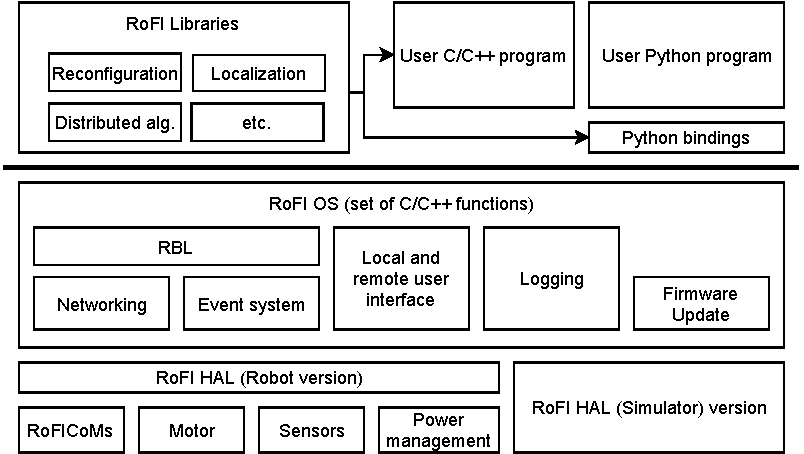
\includegraphics[width=\linewidth]{rofi_architecture.pdf}
    \caption{RoFI software architecture diagram. Diagram taken from RoFI web page\cite{rofi-web}.}
    \label{fig:hal_diagram}
\end{figure}

Diagram \ref{fig:hal_diagram} shows the RoFI software architecture.
The RoFI hardware abstraction layer (HAL) allows the user that programs RoFI modules code to not worry about the implementation details of the hardware.
Providing the same HAL interface in the simulator as well as the physical RoFI modules enables to use the same code for the physical modules and the simulator.

\subsection{Gazebo integration}

Gazebo allows extending its functionality by various plugins.
The obvious choice is to have each RoFI module have its model with a model plugin attached.
This model plugin will be simulating a processor in the physical module.

One possible design would be to compile each RoFI program into a separate plugin and each simulated RoFI module will have a plugin corresponding to the code loaded in the physical module.
This approach makes the implementation fairly simple, because it mostly just copies the physical implementation.
But there are flaws in this design as well:
\begin{itemize}
    \item When the user program would fail and terminate (e.g. because of a SIGKILL), the whole simulation would collapse, because Gazebo runs all plugins in the same process.
    \item In case of few different codes, each generated plugin would have to be available to Gazebo and specified with its own name in the world description.
    \item It eliminates (or makes really difficult) the possibility of changing the code during the simulation.
\end{itemize}

The other design, which is used in this thesis, is to make use of Gazebo topics, which allow communication between Gazebo and third party software.
In this design each module has a client side and a server side.
The server is a model plugin attached to the RoFI module, which interprets Gazebo command messages.
The client side is the users program with a small layer, that translates the RoFI HAL commands to Gazebo messages, which can be processed by the server.

The client/server separation allows to separate processes of each module and thus better imitate the physical reality.
This could also be used to imitate the limited capabilities of the microprocessor used in RoFI modules.
But there are some negative elements that have to be considered in this approach:
\begin{itemize}
    \item There is no guarantee, that the message will arrive.
    \item Even if the messages arrive, they could be delayed or reordered.
    \item There is a need for a mechanism, that will determine what the topic address will be.
\end{itemize}

\subsection{RoFICoM model}

RoFICoM (\ref{roficom}) is a key component to all RoFI modules and in most modules is featured multiple times.
Because of this and because RoFICoM has many special requirements, it's convinient to have an isolated RoFICoM model.
This also allows distributing the work from the RoFI module plugin to several RoFICoM plugins.

The communication between RoFI module plugin and RoFICoM plugins is done by Gazebo messages.
Due to Gazebo allowing only unique scoped names for models and both plugins having access to the RoFICoM model, the communication topic is the scoped name of the RoFICoM model.

\subsection{Creating modules}

The only module that the RoFI platform specifies at the time of writing is the Universal module (\ref{univ-module}).
But since RoFIbots (\ref{rofibot}) are expected to be consisting of various different RoFI modules, there is an easy way to create a new module (see Section \ref{ex-modules}).

\section{Challenges}
% difficulties in the design: what needs to be done, clients, connecting roficoms, saving world and reloading (saving plugin info to sdf), waiting

During the implementation there were few challenges to overcome.
Here are some of the more important ones with outline of the solutions and reasoning behind them.

\subsection{Distributing the RoFI modules}

The RoFI module in the simulation has no information about its id, which is used to address individual modules inside the code.
This is due to the fact, that the module can be inserted into the simulation after the start and each inserted module is the same except for the model name.
The RoFI modules plugins have to know the topic at the loading of the model, so it can communicate with rest of the simulation, so the used topic is the scoped name of the module model (as with the RoFICoM model plugin).

The client also does not know the id and the topic of the local RoFI module.
This could be solved by providing the id in each client, but this is not well scalable as many applications use the same software in all modules.

The solution utilizes a \emph{distributor} world plugin, that registers all RoFI modules in the world.
The \emph{distributor} is able to lock or free a RoFI module and give info (ids and topics) about the registered RoFI modules.

\subsection{Publishing messages from the client}

Gazebo messages use the best-effort delivery and thus may get lost.
This is a problem especially in callback based user code.
The aim was to improve the reliability by creating a publish worker, so all messages from one client are sent from the same thread.
This improved the reliability, but some messages could still get lost if the host machine is slow and multiple messages are sent at the same time.
It is possible to implement a TCP above the Gazebo messages, but that is above the scope of this thesis.

\subsection{Connecting RoFICoMs in simulation}

The biggest challenge in simulating modular robots in a general simulator is to mimic the behaviour of the docking system.
The RoFICoM has some tolerance\cite{roficom} on the area of acceptance and if connected, will perfectly align the two RoFICoMs.

An elegant solution would be to create a joint between the two RoFICoMs and connect them.
But since the models can be further apart, be rotated and misaligned at the same time, a combination of multiple joints would have to be made.
(Note that RoFICoMs connect only in 4 orientations.)
Unfortunately Gazebo is limited and uneasy to use in terms of creating joints at the runtime, so creating multiple joints becomes increasingly more difficult.

Another way is to use four points on the RoFICoM model and join these with a spring-like mechanism.
This has the advantage of only switching points that join to each other, when connecting RoFICoMs with different orientation.

\subsection{Saving and loading worlds with state}

When saving a Gazebo world, the information is saved in a SDFormat.
All the model and joint positions as well as velocities are saved, but no information about the plugins are saved.
This can lead to a situation, where a RoFICoM is half extended, which would never happen in real life.
Also the target positions, velocities or forces are forgotten and there is no telling even which movement mode was used.

A possibility would be to just say that it is undefined, but saving and reloading worlds is a useful feature, and it makes sense to keep it.
Other possibility would be to save the state of the plugin to the SDFormat.
This adds some overhead on runtime, because the SDFormat has to be updated all the time, but this overhead seems negligible.

\subsection{Waiting in the client}

Since the simulation can run at a different speed than real time (slower if the host machine is slow or even faster if Gazebo is set to do so), the standard function \code{sleep\_for} will not work as expected.

In the RoFI team we decided to provide a function \code{RoFI::wait} (that takes the waiting time and a callback) in the RoFI HAL.
Since the function \code{wait} can be called multiple times, each wait is assigned an id and sent to the local module plugin, that uses the simulation time for waiting.
Note that since every RoFI module is assigned at most one client, the wait ids can be for each client the same.


\chapter{Added utilities}

\section{World creator}
% short introduction about rofi descriptors, integration with them (world-creator)

% TODO


\chapter{Experimental evaluation}
% examples, demos
% what works, what does not - how much does it not work

\section{Creating new modules}
\label{ex-modules}

% TODO


\chapter{Conclusion}
% How I managed to make an awesome tool, that will help the world

\end{document}
